\documentclass[pdflatex,compress,mathserif]{beamer}

%\usetheme[dark,framenumber,totalframenumber]{ElektroITK}
\usetheme[darktitle,framenumber,totalframenumber]{ElektroITK}

\usepackage[utf8]{inputenc}
\usepackage[T1]{fontenc}
\usepackage{lmodern}
\usepackage[bahasai]{babel}
\usepackage{amsmath}
\usepackage{amsfonts}
\usepackage{amssymb}
\usepackage{graphicx}
\usepackage{multicol}

\newcommand*{\Scale}[2][4]{\scalebox{#1}{$#2$}}%

\setbeamertemplate{caption}[numbered]
\setbeamertemplate{section in toc}[sections numbered]

\title{Sinyal dan Sistem}
\subtitle{Bab Pengantar Sinyal dan Sistem}

\author{Dosen Pengampu:\\Mifta Nur Farid, S.T., M.T.}

\begin{document}

\maketitle

\section{Sinyal}

\begin{frame}{Sinyal}
	\begin{itemize}
		\item Sinyal direpresentasikan secara matematis sebagai fungsi dari satu atau lebih variabel bebas
	\end{itemize}
	\begin{multicols}{2}
		\begin{figure}
			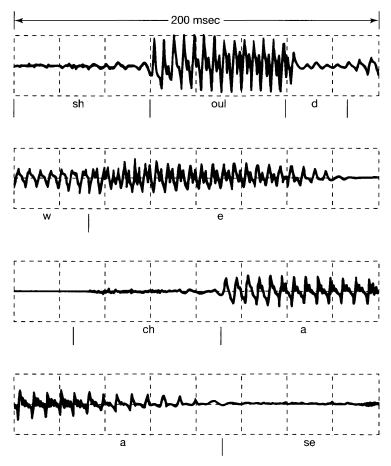
\includegraphics[width=0.5\linewidth]{img/00.sinyal_suara}
			\caption{Sinyal suara, 1 variabel (tekanan suara terhadap waktu), \textit{one-dimensional}}
		\end{figure}
		\begin{figure}
			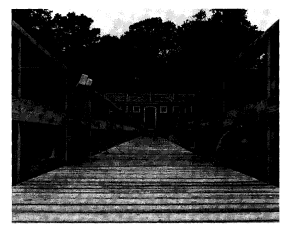
\includegraphics[width=0.7\linewidth]{img/00.sinyal_gambar}
			\caption{Gambar, 2 variabel (brightness terhadap sumbu vertikal dan horizontal), \textit{two-dimensional}}
		\end{figure}
	\end{multicols}
\end{frame}

\begin{frame}{Sinyal waktu diskret dan kontinu}
	\begin{itemize}
		\item Sinyal waktu kontinu
		\begin{itemize}
			\item Variabel bebasnya bernilai kontinu
			\item Dinotasikan dengan $ x(t) $
			\item $ t $ adalah variabel bebas
			\item Jika ada 2 variabel bebas $ \rightarrow ~ x(t,s) $, dst.
		\end{itemize}
		\item Sinyal waktu diskrit
		\begin{itemize}
			\item Variabel bebasnya bernilai diskret
			\item Dinotasikan dengan $ x[n] $
			\item $ n $ adalah variabel bebas dengan bilangan bulat
			\item Jika ada 2 variabel bebas $ \rightarrow ~ x[m,n] $ , dst.
		\end{itemize}
	\end{itemize}
\end{frame}

\begin{frame}{Sinyal waktu diskret dan kontinu}
	\begin{figure}
		\centering
		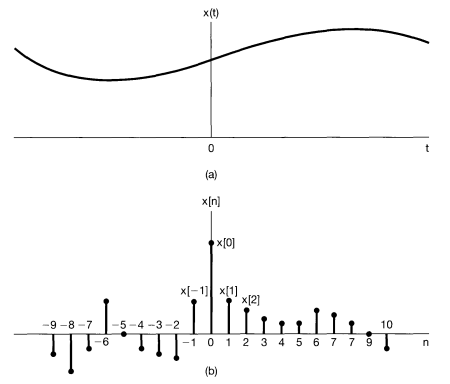
\includegraphics[width=0.5\linewidth]{img/00.representasi_grafis_dari_sinyal_waktu_kontinu_dan_diskret}
		\caption{Representasi grafis dari sinyal waktu kontinu dan diskret}
	\end{figure}
\end{frame}

\begin{frame}{Contoh sinyal waktu diskret}
	\begin{figure}
		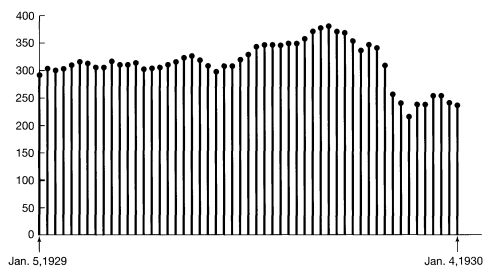
\includegraphics[height=0.7\textheight]{img/00.sinyal_waktu_diskret}
		\caption{Grafik \textit{weekly stock market index} adalah contoh sinyal waktu diskret}
	\end{figure}
\end{frame}

\begin{frame}{Contoh sinyal waktu kontinu}
	
	\begin{figure}
		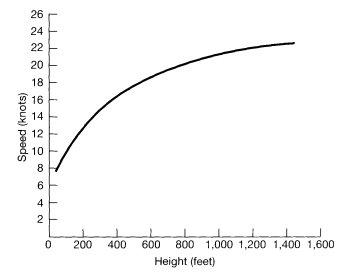
\includegraphics[height=0.7\textheight]{img/00.sinyal_waktu_kontinu}
		\caption{Grafik profil kecepatan angin adalah contoh sinyal waktu kontinu}
	\end{figure}
\end{frame}


\section{Sistem}

\begin{frame}{Sistem}
	\begin{itemize}
		\item Sistem berfungsi untuk memproses sinyal
		\item Sistem linear / non-linear
		\item Sistem time-invariant / time-varying
		\item Fokus kita nantinya di linear time-invariant (LTI)
	\end{itemize}
	\begin{figure}
		\centering
		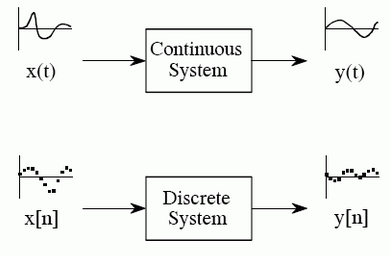
\includegraphics[width=0.5\linewidth]{img/00.sistem}
		\caption{Terminologi sinyal dan sistem}
	\end{figure}
\end{frame}

\begin{frame}{Contoh sistem diskret}
	\begin{figure}
		\centering
		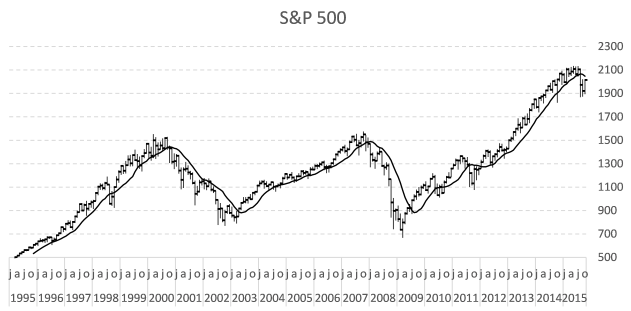
\includegraphics[height=0.7\textheight]{img/00.proses_sinyal_diskret}
		\caption{Market trend}
	\end{figure}
\end{frame}

\begin{frame}{Contoh sistem kontinu}
	\begin{figure}
		\centering
		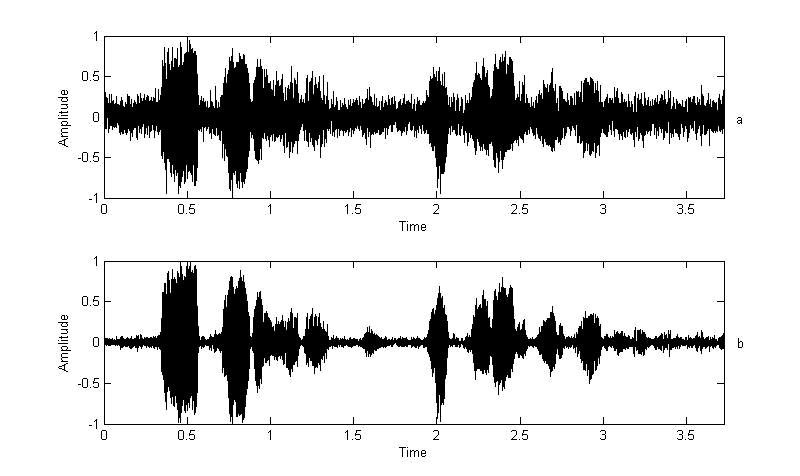
\includegraphics[height=0.7\textheight]{img/00.proses_sinyal_kontinu}
		\caption{Menghilangkan noise dari suara rekaman (gambar atas = suara dengan noise, gambar bawah = noise sudah dihilangkan)}
	\end{figure}
\end{frame}

\begin{frame}{Contoh sistem yang memproses sinyal multi-dimensional}
	\begin{multicols}{2}
		\begin{figure}
			\centering
			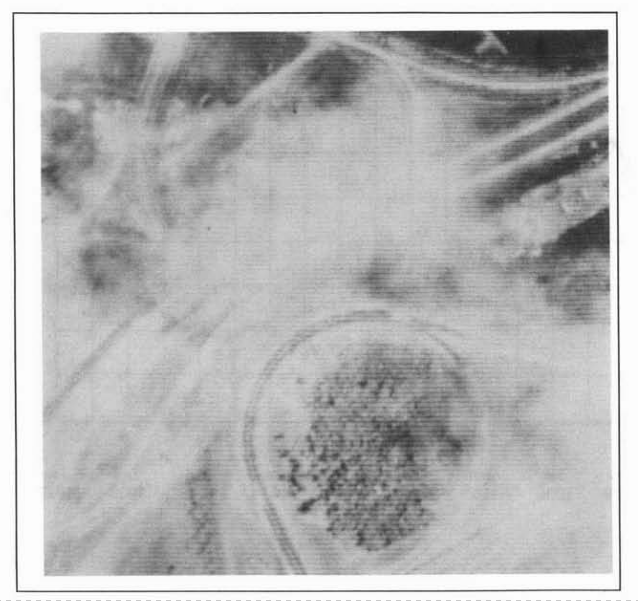
\includegraphics[width=\linewidth]{img/00.foto_jalan_berawan}
			\caption{Foto jalan berawan}
		\end{figure}
		\vfill\null
		\columnbreak
		\begin{figure}
			\centering
			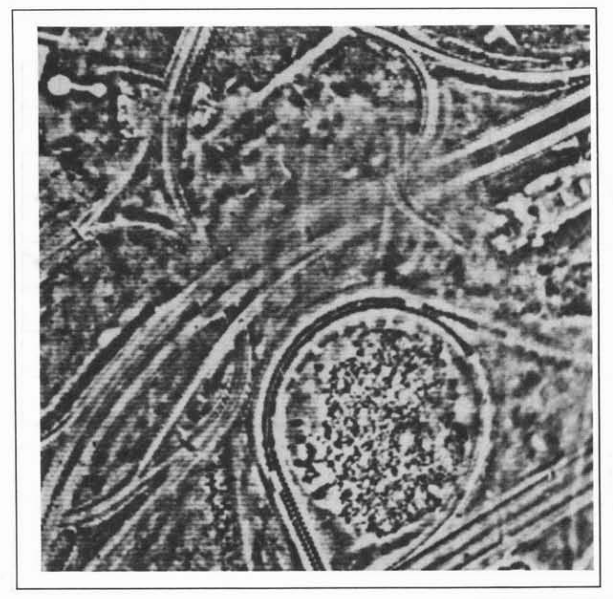
\includegraphics[width=\linewidth]{img/00.foto_jalan_awan_hilang}
			\caption{Hasil pemrosesan menghilangkan awan}
		\end{figure}
	\end{multicols}
\end{frame}
\begin{frame}{Interkoneksi antar sistem}
	\begin{itemize}
		\item Terkadang antara satu sistem dengan sistem lainnya saling terinterkoneksi
		\item Interkoneksi antar sistem :
		\begin{enumerate}
			\item Seri
			\item Paralel
			\item \textit{Cascade} (Bertingkat)
			\item \textit{Feedback} (Umpan-balik) $ \leftarrow $ akan menjadi topik utama dalam kuliah ini
		\end{enumerate}
	\end{itemize}
\end{frame}

\begin{frame}{\textit{Domain} (ranah) dalam analisis dan representasi}
	\begin{enumerate}
		\item \textit{Time-domain}(ranah waktu)
		\begin{itemize}
			\item $ x(t) $
			\item $ x[n] $
		\end{itemize}
		\item \textit{Frequency-domain} (ranah frekuensi)
		\begin{itemize}
			\item \textit{Fourier transform}
			\item \textit{Laplace transform}
			\item \textit{$ \mathcal{Z} $-Transform}
		\end{itemize}
	\end{enumerate}
\end{frame}

\begin{frame}{\textit{Domain} (ranah) dalam analisis dan representasi}
	\begin{figure}
		\centering
		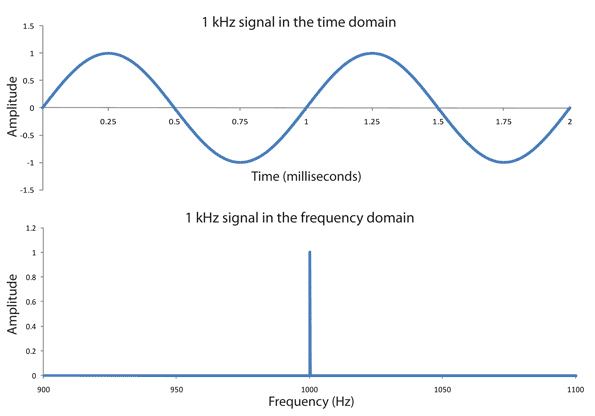
\includegraphics[width=0.7\linewidth]{img/00.TimeDomain}
		\caption{Contoh sinyal ranah waktu (atas) dan ranah frekuensi (bawah)}
	\end{figure}
\end{frame}

\begin{frame}
	\frametitle{Bahan Bacaan Mandiri}
	\begin{enumerate}
		\item Oppenheim, A. V., Willsky, A. S. \& Nawab, S. H., (1997). Signal and Systems, Second Edition. New Jersey: Prentice Hall of India.
		\begin{itemize}
			\item Chapter 1, p. 1
			\item Section 1.0, Introduction, p. 1
			\item Section 2.1, Continuous-time and Discrete-time signals, pp. 1-7
		\end{itemize}
	\end{enumerate}
\end{frame}
\end{document}
